% Example LaTeX document for GP111 - note % sign indicates a comment
\documentclass[12pt,a4paper,oneside]{article}
\usepackage{lmodern}
\usepackage[french]{babel}
\usepackage[T1]{fontenc}
\usepackage[utf8]{inputenc}
\usepackage{graphicx}
\usepackage{hyperref}
\usepackage{float}
\usepackage[ruled,vlined]{algorithm2e}


% Default margins are too wide all the way around. I reset them here
\setlength{\topmargin}{-.5in}
\setlength{\textheight}{9in}
\setlength{\oddsidemargin}{.125in}
\setlength{\textwidth}{6.25in}

\hypersetup{
    unicode=false,          % non-Latin characters in Acrobat’s bookmarks
    pdftoolbar=true,        % show Acrobat’s toolbar?
    pdfmenubar=true,        % show Acrobat’s menu?
    pdffitwindow=false,     % window fit to page when opened
    pdfnewwindow=true,      % links in new window
    colorlinks=true,       % false: boxed links; true: colored links
    linkcolor=black,          % color of internal links (change box color with linkbordercolor)
    citecolor=green,        % color of links to bibliography
    filecolor=magenta,      % color of file links
    urlcolor=cyan,          % color of external links
    linktoc=page
}

\begin{document}

\begin{titlepage}
\begin{flushright}
           
\includegraphics[scale=0.30]{../images/univorleans.png}\\ 
                      Département Informatique
\end{flushright}
\vspace{30mm}
\begin{center}
\textbf{\huge{Documentation technique SIG }}\\
\vspace{8mm}
\begin{large}
	\textit{Jordan FONTORBE}\\
	\textit{Willy FRANÇOIS}\\
	\textit{Jérémy MOROSI}\\
	\textit{Jean-Baptiste PERRIN}
\end{large}

\end{center}
\begin{figure}[b!]
\begin{flushright}
~~\\ ~~\\ ~~\\ ~~\\ ~~\\ ~~\\ ~~\\
\large{Année : 2013-2014}
\end{flushright}
\end{figure}
\end{titlepage}

\newpage

\tableofcontents
\newpage

\section{Analyse}

\subsection{Commun}
\subsubsection{Package geometry}
L'arbre de décision, qui permet de localiser le bâtiment contenant un point donné, est composé d'un noeud racine qui se découpe en quatre noeuds par rapport à son centre, qui se découpent également chacun en quatre noeuds par rapport à leur centre, jusqu'à atteindre les feuilles.\\

Un noeud est représenté par la classe \texttt{Node}, et une feuille par la classe \texttt{Leaf}. Ces deux classes implémentent l'interface \texttt{INode} qui propose la méthode de localisation du point \texttt{BoundingBox locate(double x, double y)}. Comme la classe \texttt{BoundingBox} est utilisée pour stocker le rectangle englobant et l'identifiant d'un bâtiment, on peut considérer que la méthode \texttt{locate} retourne le bâtiment contenant le point donné. Le rectangle englobant est tout simplement le plus petit rectangle contenant l'ensemble des points du polygone formant le bâtiment.\\

Un noeud contient des coordonnées \texttt{x} et \texttt{y}, qui correspondent à son centre, et les quatre sous-noeuds qui le composent. Ces coordonnées servent à savoir où se situe le point donné par rapport au centre du noeud, et si il faut appeler la méthode \texttt{locate} sur le sous-noeud en haut à gauche, en haut à droite, en bas à gauche, ou en bas à droite.

Une feuille contient la liste des bâtiments dont le rectangle englobant intersecte sa zone. Par exemple, si l'arbre couvre une zone dont le point en haut à gauche est $(0, 0)$, et le point en bas à droite est $(1, 1)$, et qu'il possède un noeud racine qui se décompose en quatre feuilles, alors le centre du noeud est le point $(0.5, 0.5)$, et la feuille en haut à gauche contient la liste des bâtiments dont le rectangle englobant intersecte le rectangle d'origine $(0, 0)$, de largeur $0.5$, et de hauteur $0.5$.\\

Avec cette structure, au lieu de devoir tester tous les bâtiments existants, on commence par récupérer la feuille qui contient le point, et ainsi, on est sûr de ne tester que les bâtiments qui intersectent la zone représentée par la feuille et qui ont une chance de contenir le point. De plus, on ne teste pas si un bâtiment contient le point par rapport au polygone qui représente le bâtiment, mais par rapport à son rectangle englobant.

\`{A} noter que si une une feuille ne contient aucun bâtiment, alors elle remplacée par \texttt{NullNode.NULL} dans l'arbre. De même, si les quatre sous-noeuds d'un noeud correspondent à \texttt{NullNode.NULL}, alors le noeud est remplacé par \texttt{NullNode.NULL}. Ainsi, un noeud n'existe dans l'arbre que si il possède au moins une feuille qui contient des bâtiments. Par conséquent, l'arbre prend considérablement moins de place en mémoire, et la localisation d'un point s'arrête immédiatement si le point se situe dans une zone sans bâtiments.
\subsubsection{Package data}
Le package \textbf{data} contient le modèle des données ainsi que les fonctions (SQL et XML) nécessaire au prétraitement des données.
\paragraph{Le modèle : \\}
Notre modèle correspond à la structure de notre base de données. Nous avons choisi de ne garder que les nœuds, les trous, les routes, les bâtiments, les bassins et les forêts. Ainsi nous retrouvons : \\
\renewcommand{\labelitemi}{$\bullet$}
\begin{itemize}
\item une classe \textbf{Node} contenant un \textit{id}, une \textit{latitude} et une \textit{longitude}. Cette classe caractérise un point de la carte et va permettre avec ses coordonnées de construire une route, un bâtiment, un bassin ou une forêt.
\item une classe \textbf{Road} contenant un \textit{id}, un \textit{nom} (pas obligatoire),  un \textit{type} (route secondaire, chemin, route piétonne, etc.), la liste des nœuds qui la constitue et sa \textit{géométrie}.
\item une classe abstraite \textbf{Structure} possédant un \textit{id}, un {nom} (pas obligatoire), la liste des nœuds qui constitue cette structure, sa géométrie ainsi que la liste de ses trous (peut être vide). Les classes héritant de \textbf{Structure} sont :
	\begin{itemize}
	\item la classe \textbf{Building}. Elle représente un bâtiment et à en plus une liste de tous ses nœuds proches (hors ceux constituant le bâtiment).
	\item la classe \textbf{Basin} décrivant un bassin (lac, étang, etc.)
	\item la classe \textbf{Forest} décrivant une forêt.
	\item la classe \textbf{Hole} décrivant un trou d'une structure. Elle possède en plus l'id de la structure à laquelle il appartient.
	\end{itemize}
\end{itemize}
Le modèle est représenté par le schéma ci-dessous :\\

\begin{figure}[H]
\centering
\resizebox{\linewidth}{!}{
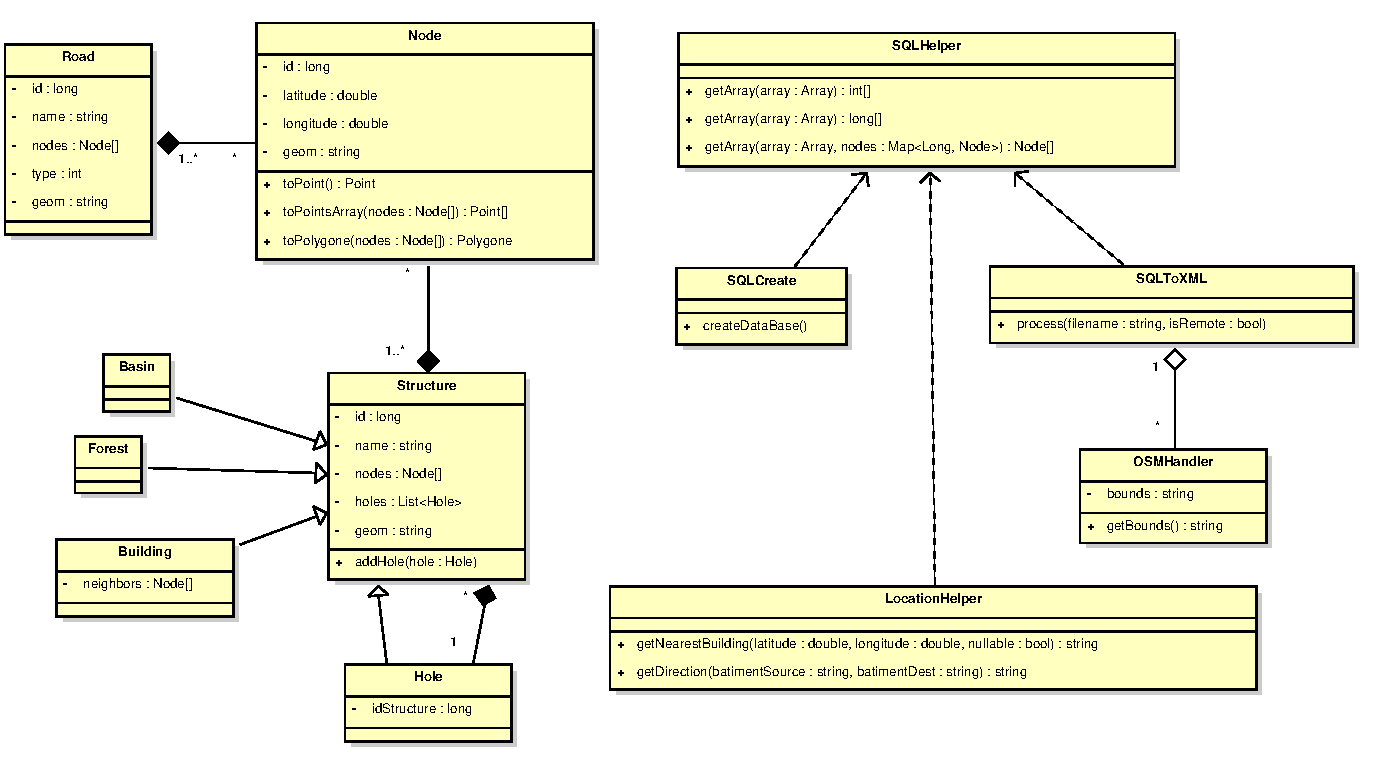
\includegraphics{../images/communData.pdf}
}
\caption{Modèle}
\end{figure}

\paragraph{Le pré-traitement : \\}
Une étape de pré-traitement à été nécessaire. En effet lorsque nous avons récupérer les données \textit{OpenStreetMap} et importé dans une base de données (à l'aide de l'outil \textit{osm2pgsql}), nous avons dû récupérer seulement les informations qui nous étaient utiles. Ainsi nous avons créé 4 nouvelles tables correspondant à notre modèle (sig1337\_nodes, sig1337\_roads, sig1337\_holes et sig1337\_structures) avec seulement les informations nécessaire (coordonnées, géométrie, nom, ...). Cette génération se fait à l'aide de la classe \textbf{SQLCreate} du package \textbf{data.sql}. \\
Ensuite, les données vont être récupérées et parsée en XML. On retrouvera notamment les tags :
\begin{itemize}
\item \textbf{bassin}, contenant un nom, une liste de voisins, et les triangles permettant sa construction en \textit{OpenGL}.
\item \textbf{foret}, contenant un nom, une liste de voisins, et les triangles permettant sa construction en \textit{OpenGL}.
\item \textbf{batiment}, contenant un nom, une liste de voisins, et les triangles permettant sa construction en \textit{OpenGL}.
\item \textbf{route}, contenant la liste des points la décrivant et son type (chemin ou route pour une réprésentation différent sur la carte).
\end{itemize}

\newpage

\subsection{WebService}
Afin de permettre une utilisation de l'application en mode "remote", un \textit{WebService} a été mis en place. Aucune donnée (comme les bâtiments, les routes, l'arbre de décision) n'étant stockée sur le téléphone dans ce mode, c'est l'appel aux méthodes de ce \textit{WebService} qui va nous permettre de récupérer toutes les données nécessaires. \\
Il permet entre autre d'avoir accès à trois méthodes :\\
\begin{itemize}
\item Une méthode permettant de récupérer les informations de la carte au format XML, c'est-à-dire les nœuds, les routes et les structures ainsi que l'arbre de décision. Cette méthode sera appelée au lancement de l'application en mode "remote". Elle est accessible à partir de l'URL : http://\textit{IP\_ADRESS}:\textit{PORT}/WebService/service/map. La définition de cette méthode est présente dans la classe \textbf{MapService}.
\item Une méthode permettant à partir d'une latitude et d'une longitude, de récupérer le plus proche bâtiment. Elle sera appelée dans l'application Android, lors d'un appuie sur une zone de la carte afin de pouvoir sélectionner un bâtiment comme point de départ ou d'arrivée pour un itinéraire. Cette méthode est accessible à partir de l'URL : http://\textit{IP\_ADRESS}:\textit{PORT}/WebService/service/location/building/\{lat\}/\{lon\}. Elle est définie dans la classe \textbf{LocationService}.
\item Une méthode permettant à partir de l'identifiant d'un bâtiment de départ et de l'identifiant d'un bâtiment d'arrivée de retourner un itinéraire (au format JSON). La réponse renvoie la liste des coordonnées à parcourir. Cette méthode sera appelée lors de la demande de calcul d'un itinéraire par l'utilisateur et est accessible à partir de l'URL : http://\textit{IP\_ADRESS}:\textit{PORT}/WebService/service/location/direction/\{id départ\}/\{id arrivée\}. Cette méthode est définie dans la classe \textbf{LocationService}.\\
\end{itemize}

La méthode récupérant le XML décrivant la carte étant la plus longue, c'est un tâche asynchrone qui l'appel. Les deux autres méthodes étant relativement rapide (une seconde environ), on attend la réponse du WebService (avec une limite fixée à 3 secondes pour ne pas bloquer l'application trop longtemps). 

\newpage

\subsection{Android}

\subsubsection{Partie commune}

Afin de faciliter l'implémentation de la version locale et distante du projet Android,
nous avons défini un socle commun aux deux versions.

Une interface \textit{ISIG1337} contenant des méthodes nécessaire à l'application telles que load,
getStructureId, getStructureName et getItineraire.
Cette interface est directement implémentée par la classe abstraite \textit{SIG1337Base},
fournissant quelques méthodes de l'interface.

\begin{figure}[H]
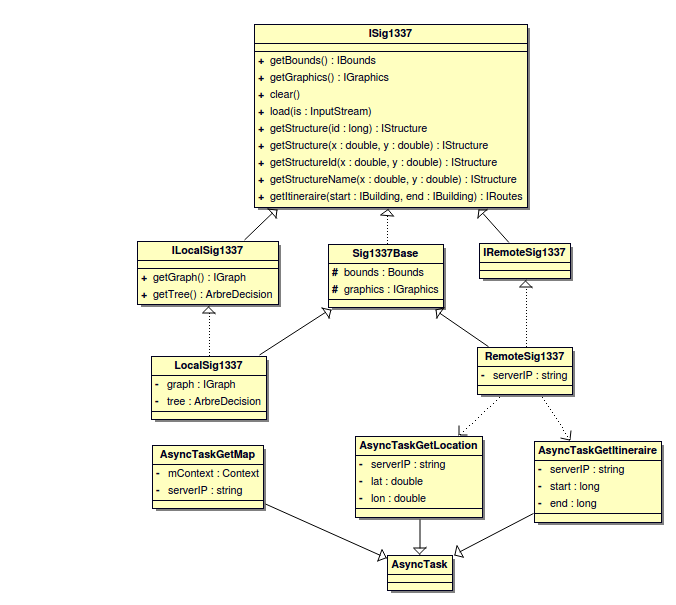
\includegraphics[width=1\textwidth]{../images/androidSIG.png}
\caption{Activités Android}
\end{figure}


\subsubsection{Version locale}

Pour la version locale, nous avons créé \textit{LocalActivity} qui hérite de \textit{ActivityBase}.
Elle contient une instance de \textit{LocalSIG1337}, qui hérite de \textit{SIG1337Base} et qui implémente \textit{ILocalSIG1337}.
Cette dernière possède les méthodes getGraph et getTree, permettant respectivement de récupérer le graphe et l'arbre de décision.

La méthode loadSIG1337() qui doit charger le SIG va charger le xml qui avait été généré précédemment dans le projet \textit{Commun}
et qui a été placée dans les fichiers de l'application.
Ce fichier, en version locale, contient la carte au format xml, le graphe et l'arbre de décision.

Lorsqu'on touche un bâtiment sur la carte, un calcul est fait sur l'arbre de décision qui renvoie finalement le nom du dit bâtiment.

Pour le calcul d'itinéraire, une fois les deux bâtiments sélectionnés via \textit{ItineraireActivity} et le bouton validé,
l'application fait appel au graphe afin de calculer l'itinéraire entre ces deux bâtiments.


\subsubsection{Version distante}

Pour la version distante, nous avons créé \textit{RemoteActivity} qui hérite de \textit{ActivityBase}.
Elle contient une instance de \textit{RemoteSIG1337}, qui hérite de \textit{SIG1337Base} et possède un attribut serverIP,
permettant d'avoir l'adresse du serveur.

La méthode loadSIG1337() qui doit charger le SIG fait appel à une instance de la classe \textit{AsyncTastGetMap},
qui hérite de \textit{AsyncTask}.
Cette tâche asynchrone fait appel, via une requête http, au WebService hébergé sur un serveur distant.
Le serveur renvoie la carte au format xml allégé de l'arbre de décision.
Une fois la réponse du serveur récupérée, la méthode createMap de l'activité est appelée et charge la carte en mémoire.

Lorsqu'on touche la carte un court instant, une requête est envoyée au WebService,
via une instance de la classe \textit{AsyncTaskGetLocation},
qui va récupérer les informations de base du bâtiment le plus proche de l'endroit que l'on a touché, au format JSON.
La tâche asynchrone va récupérer ce JSON, le parser et afficher un Toast avec le nom du bâtiment.

Pour le calcul d'itinéraire, une fois les deux bâtiments sélectionnés via \textit{ItineraireActivity} et le bouton validé,
l'application fait appel à une instance de \textit{AsyncTaskGetItineraire},
qui va demander au WebService de calculer le chemin le plus court entre les deux bâtiments.
La réponse est renvoyée au format JSON afin de pouvoir être parsée facilement via l'application.
Celle\-ci va ensuite ajouter un chemin du bâtiment de départ au bâtiment d'arrivée sur la carte.




\newpage

\section{Solutions techniques retenues}

Au départ, nous voulions implémenter le \texttt{Randomized Incremental Algorithm} pour la génération de l'arbre de décision. Cet algorithme prend en paramètre un ensemble de segments, et retourne un découpage en trapèzes ainsi qu'un arbre de recherche qui permet de savoir dans quel trapèze se trouve un point donné.

Une première difficulté était l'implémentation de l'algorithme. L'algorithme nécessite que chaque trapèze connaisse ses deux voisins de gauche et de droite. Le livre décrit comment modifier les trapèzes et l'arbre de recherche suivant si le segment ajouté intersecte un ou plusieurs trapèzes, mais il n'indique jamais comment gérer les voisins. De plus, pour le cas simple où le segment ajouté occupe un seul trapèze, le livre indique bien à la fin qu'il faut gérer les cas où le point à gauche (ou à droite) du segment est aussi le point à gauche (ou à droite) du trapèze, mais ne dit pas comment. Les explications du livre paraissent simples, mais on se retrouve à devoir gérer un bon nombre de cas et à complexifier le code à cause de cette notion de voisins.

Une seconde difficulté était qu'il n'y a pas de notion d'être à l'intérieur où à l'extérieur d'un polygone. L'algorithme génère un découpage en trapèzes et un arbre de recherche qui nous retourne le trapèze dans lequel se trouve un point. Cependant, on ne sait pas si ce trapèze est à l'intérieur d'un polygone ou bien à l'extérieur. On ne sait pas non plus à quel polygone appartient le trapèze. D'ailleurs, il n'y a pas de notion de polygone ou de zone dans l'algorithme puisqu'il prend une liste de segments en paramètre. Il est donc nécessaire de faire un pré-traitement ou post-traitement pour labéliser les trapèzes.\\

Plutôt que de rester sur une implémentation incorrecte de cet algorithme, nous avons opté pour une version, certes moins optimisée, mais plus simple et fonctionnelle (voir Algorithm \ref{algoarbre}). Puisque la complexité pour localiser un point vient du fait que les bâtiments sont des polygones et qu'il y a beaucoup de bâtiments à tester, nous avons fait deux choses.

Premièrement, nous avons calculé un rectangle englobant pour chaque bâtiment. Ainsi, plutôt que de devoir parcourir tous les points d'un polygone pour savoir si le point en question est à l'intérieur, il nous suffit de tester si il est à l'intérieur du rectangle.

Deuxièmement, pour ne pas avoir à tester chaque rectangle englobant à chaque fois, nous avons généré un arbre de recherche. On commence avec un noeud qui fait la taille de la carte et qui contient une liste de tous les bâtiments. On divise ce noeud en deux horizontalement et verticalement de manière à obtenir quatre nouveaux noeuds. On donne à chaque nouveau noeud une nouvelle liste qui ne contient que les bâtiments du noeud initial dont les rectangles englobants intersectent le rectangle représenté par le noeud. Le centre du noeud initial nous sert à savoir dans quel sous noeud se trouve le bâtiment contenant le point recherché. On continue à diviser les noeuds un certains nombre de fois, suffisamment pour que chaque noeud ne contienne plus qu'un nombre réduit de bâtiments et pour que l'arbre ne prenne pas trop de place en mémoire.

L'arbre ainsi obtenu nous permet d'optimiser la localisation d'un point en réduisant le nombre de bâtiments, et donc de rectangles, à tester grâce au découpage de la carte en zones de tailles égales.\\

\begin{algorithm}[H]
 \KwData{A set of buildings $buildings$, the depth of the tree $depth$}
 \KwResult{The decision tree}
$boundingBoxes$ $\gets$ an empty list of bounding boxes\;
\For{each building in $buildings$}{
  add the bounding box of the building to $boundingBoxes$\;
}
calculate the smallest bounding box containing all the buildings\;
$minX$, $minY$, $maxX$, $maxX$ $\gets$ coordinates of the bounding box\;
$root \gets split(minX$, $minY$, $maxX$, $maxY$, $depth$, $boundingBoxes)$\;
\Return $Tree(root)$\;
 \caption{create\label{algoarbre}}
\end{algorithm}
~\\
\begin{algorithm}[H]
 \KwData{A rectangle $minX$, $minY$, $maxX$, $maxY$, the depth of the tree $depth$, a list of bounding boxes $boundingBoxes$}
 \KwResult{A node}
$list$ $\gets$ an empty list of bounding boxes\;
\For{each bounding box in $boundingBoxes$}{
  \If{the bounding box intersect the rectangle}{
    add the bounding box to $list$\;
  }
}
\uIf{$list$ is empty}{
  \Return $null$\;
} \uElseIf{$depth = 0$}{
 \Return $Leaf(list)$\;
} \Else {
  $cX$, $cY$ $\gets$ the center of the rectangle\;
  $depth \gets depth - 1$\;
  $topLeft \gets split(minX$, $minY$, $cX$, $cY$, $depth$, $list)$\;
  $topRight \gets split(cX$, $minY$, $maxX$, $cY$, $depth$, $list)$\;
  $bottomLeft \gets split(minX$, $cY$, $cX$, $maxY$, $depth$, $list)$\;
  $bottomRight \gets split(cX$, $cY$, $maxX$, $maxY$, $depth$, $list)$\;
  \eIf{all the nodes are $null$} {
    \Return $null$\;
  } {
    \Return $Node(topLeft$, $topRight$, $bottomLeft$, $bottomRight$, $cX$, $cY)$\;
  }
}
 \caption{split}
\end{algorithm}

\subsection{OpenGL}

Dans un soucis d'optimisation de l'affichage en OpenGL, nous avons regroupé les éléments similaires (bâtiments, bassins, routes, ...) et de même couleur de manière à n'avoir qu'un seul \texttt{vertex buffer} par type d'élément et par couleur. Ainsi, lorsque nous voulons afficher, par exemple, les bâtiments, nous donnons directement le \texttt{buffer} contenant tous les triangles des bâtiments à la fonction \texttt{glDrawArrays}. Et puisque le \texttt{buffer} ne contient que des éléments de même couleur, nous n'avons pas besoin de \texttt{color buffer}. De même, dans le cas des bâtiments, nous n'avons pas besoin d'\texttt{index buffer}.

\section{Déploiement}

\appendix
\end{document}
